\documentclass[10pt,a4paper,oneside,twocolumn]{article} %type of the document + options [(no)titlepage, landscape, one/twocolumn,...]

    \usepackage{float}	% for floating figures (putting them anywhere we want
    \usepackage{amsmath}	% for maths
    \usepackage{graphicx}	% jpg
    \usepackage{hyperref}
    \usepackage{textcomp}
    \usepackage{verbatim}	% use of \begin{comment}
    \usepackage{pgfplots}	% use of pgf plots
    \usepackage{multicol}
  %  \usepackage[top=2cm, bottom=2cm, left=2cm, right=2cm]{geometry} %margins
    \usepackage{sidecap}	% for side captions
    \restylefloat{table}	% floating figures(Tables)
    \usepackage{caption}
    \captionsetup{justification=justified}

    \numberwithin{equation}{section} %permits numbering within sections instead of globally
\begin{document}

\title{\huge{\textbf{Report}}\\
	\vspace{0.5cm}
	\Large{\textit{\'Ecole Polytechnique F\'ed\'erale de Lausanne, Switzerland}}}
\author{\large{Florian + Dariush}}

\begin{titlepage}
 \maketitle
\thispagestyle{empty}
\end{titlepage}

\section{Introduction}
    Introduction to the article goes here \\
\section{The Model}
    \begin{enumerate}
	\item
	    \begin{figure}[!h]
		    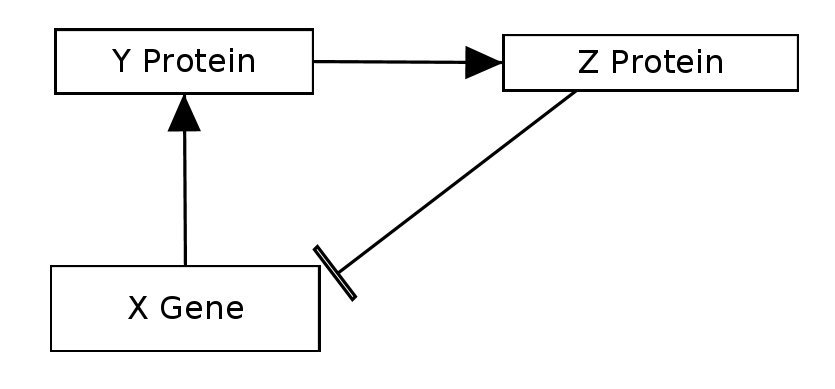
\includegraphics[scale=0.5]{sketch.png}
		    \caption{Sketch of that thing blabla}
	    \end{figure}
	\item X : mRNA concentration \\
	Y : protein concentration \\
	K : coupling strength\\
	etc\\

	\item assumptions : cell-cell interaction and light act independently, expressivity = 1, ...

    \end{enumerate}

\end{document}
